\documentclass[14pt]{extarticle}
\usepackage[utf8]{inputenc}
\usepackage[T1]{fontenc}
\usepackage[spanish,es-lcroman]{babel}
\usepackage{amsmath}
\usepackage{amsthm}
\usepackage{physics}
\usepackage{tikz}
\usepackage{float}
\usepackage[autostyle,spanish=mexican]{csquotes}
\usepackage[per-mode=symbol]{siunitx}
\usepackage{gensymb}
\usepackage{multicol}
\usepackage{enumitem}
\usepackage[left=2.00cm, right=2.00cm, top=2.00cm, 
     bottom=2.00cm]{geometry}
\usepackage{makecell}

\newcommand{\textocolor}[2]{\textbf{\textcolor{#1}{#2}}}
\sisetup{per-mode=symbol}
\DeclareSIUnit[number-unit-product = {\,}]\cal{cal}
\DeclareSIUnit{\dB}{dB}
%\renewcommand{\questionlabel}{\thequestion)}
\decimalpoint
\sisetup{bracket-numbers = false}

\title{\vspace*{-2cm} Actividad - Ejercicios Hidrodinámica \vspace{-5ex}}
\date{}

\begin{document}
\maketitle

Esta actividad otorgará hasta \textbf{5 puntos} de Evaluación Continua.
\vspace*{0.5cm}

\textbf{Instrucciones: }
\begin{itemize}
\item Anota tu nombre en cada hoja que ocupes para resolver los ejercicios.
\item Identifica el ejercicio que resuelves.
\item Resuelve detalladamente cada ejercicio, en caso de que no se tenga el desarrollo, no se tomará en cuenta como ejercicio completo, revisa con cuidado el manejo de las unidades.
\item En caso de plagios, se cancelarán todos los trabajos involucrados.
\end{itemize}


\section*{Ejercicios a resolver.}

\begin{enumerate}
\item Calcula el tiempo que tardará en llenarse un tanque cuya capacidad es de \SI{8}{\cubic\meter} al suministrarle un gasto de \SI{60}{\liter\per\second}.
\item Determina el diámetro que debe tener una tubería, para que el gasto sea de \SI{0.5}{\cubic\meter\per\second} a una velocidad de \SI{6}{\meter\per\second}.
\item Por una tubería de \SI{3.9}{\centi\meter} de diámetro circula agua a una velocidad cuya magnitud es de \SI{4.5}{\meter\per\second}. En la parte final de la tubería hay un estrechamiento y el diámetro es de \SI{2.25}{\centi\meter}. ¿Qué magnitud de velocidad llevará el agua en este punto?
\item Por la tubería que se muestra en la siguiente figura, fluyen \SI{0.11}{\cubic\meter\per\second} de gasolina, si la presión antes de la reducción es de \SI{415}{\kilo\pascal}.
\begin{figure}[H]
    \centering
    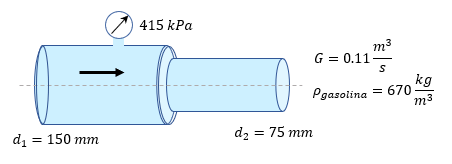
\includegraphics{Imagenes/Problema_02.png}
    \caption{Esquema para el problema 4.}
\end{figure}
Calcula la presión en la tubería de \SI{75}{\milli\meter} de diámetro.
\item Determina a qué altura se debe abrir un orificio de un estanque, para que el líquido salga con una velocidad de \SI{9}{\meter\per\second}.
\end{enumerate}
\end{document}